% coucou

\section{Results}
This section presents the different calculation results obtained by the different codes and the estimators distribution defined in the previsous section. The assumption made here is to suppose that introducing a physic model like a FLM into a fuel cycle simulation represents better the reality than no model like a FF for all plutonium fresh compositions. Our calculations don't validate any model and the purpose of this work is not to compare FLMs between them and select one. It tries to assess the need of FLM for some local or global conclusion in fuel cycle studies by estimating bias on elementary calculations. Actually, our work aims to give conclusions on the use of FF model.   

\subsection{Pressurized Water Reactor}

\subsubsection{Output analyses}
Figure~\ref{fig:PWR_MOX_FLM_Pu} presents the plutonium fraction at BOC predicted by each FLM and the plutonium fraction at EOC deduced by each software. As all FLM are different, the BOC plutonium fractions differ from a software from another. The wider prediction is given by the CLASS code that predicts plutonium fraction from 4\% until more that 15\%. This range is a direct consequence of the plutonium sampling used for this work. 15\% is clearly unrealistic but some of the plutonium isotopic composition sampled are not either by containing a low amount of fissile. That's why the FLMs may reach such high values.    

\begin{figure}[h]
	\begin{center}
		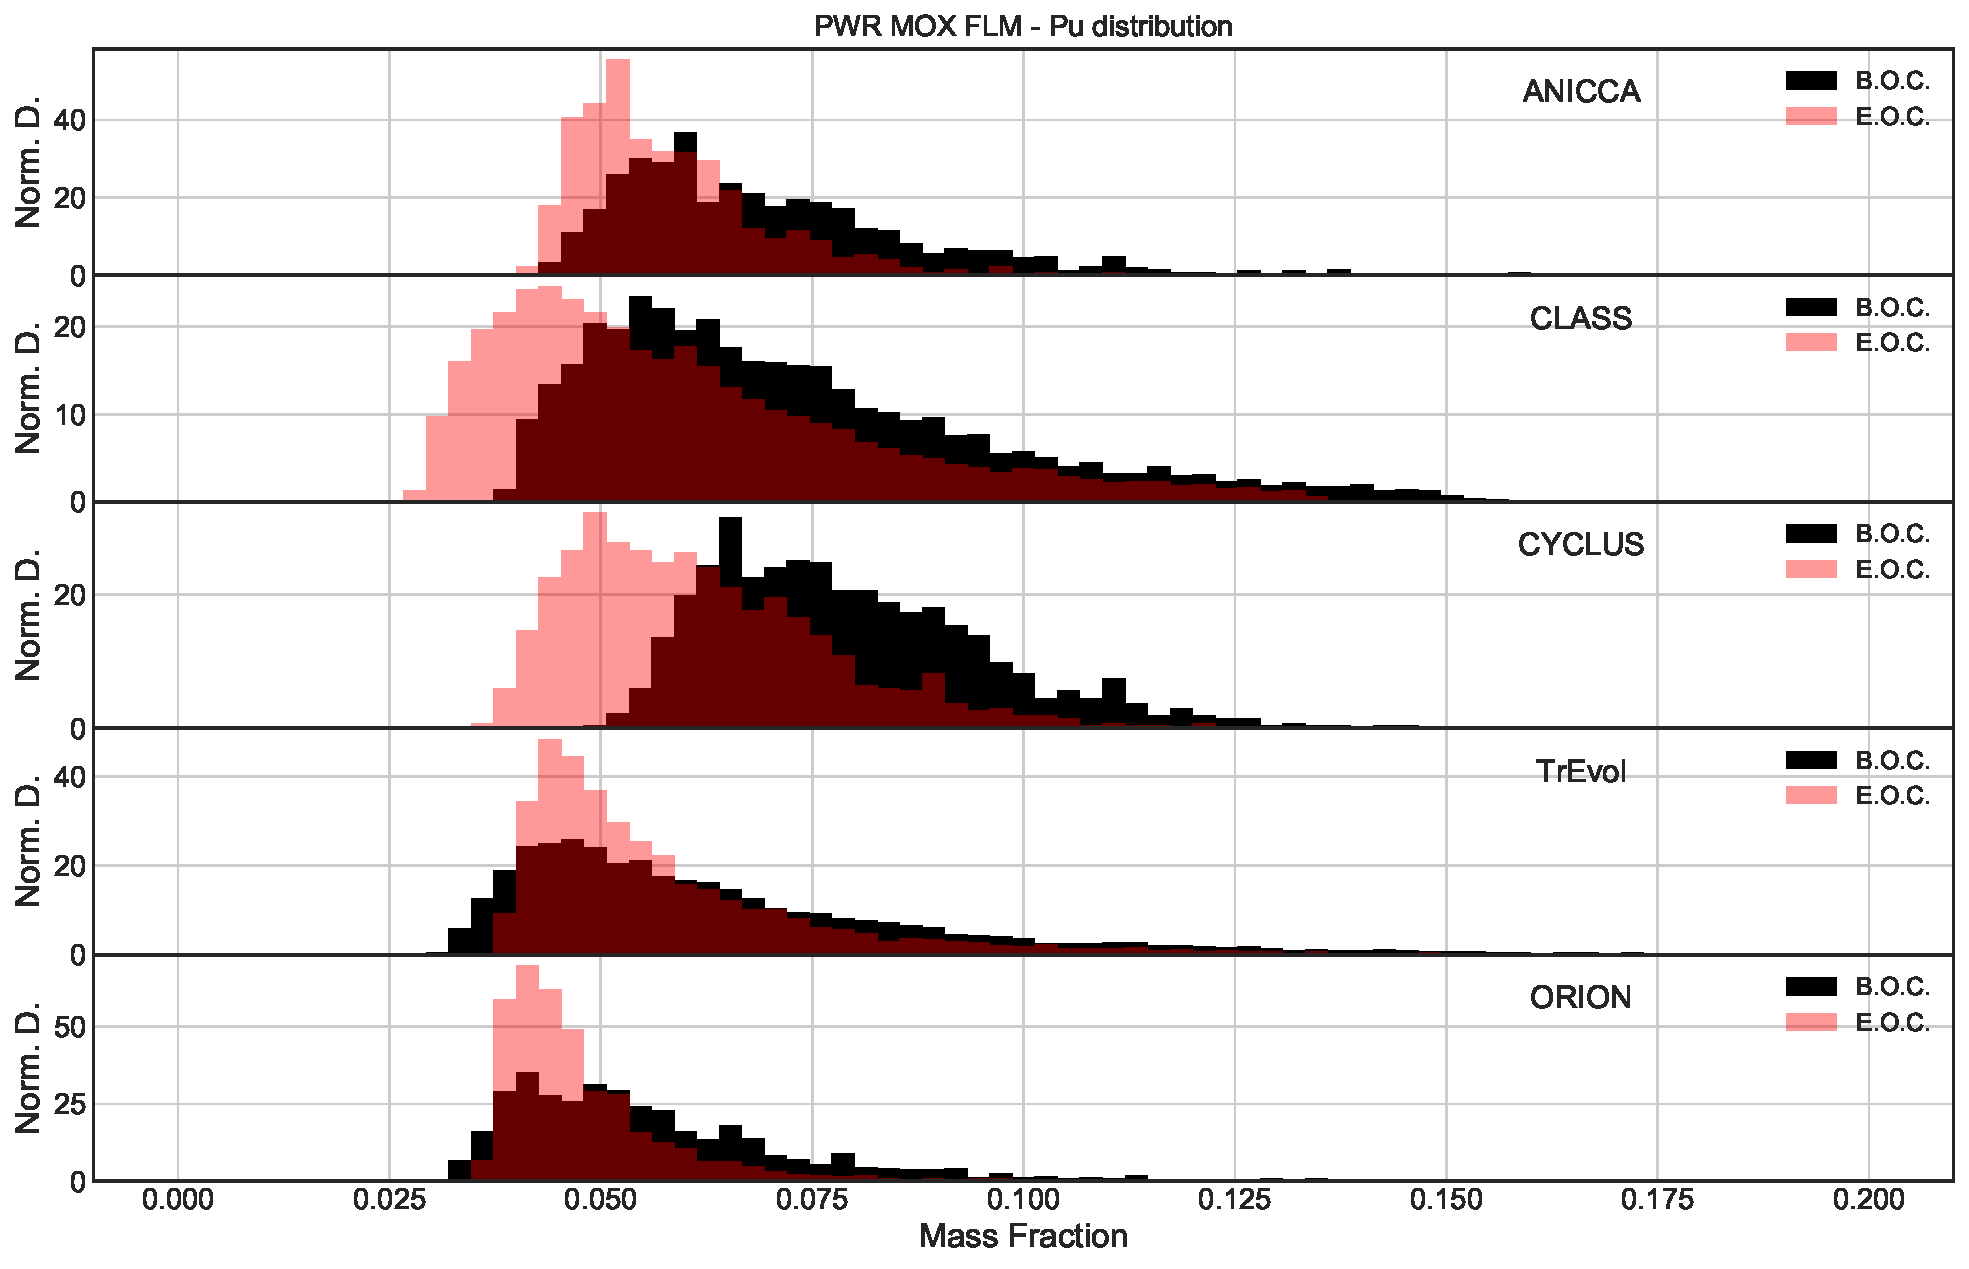
\includegraphics[width = 0.99\textwidth]{../../Feature_1/RAW_DATA/FIG/PWR_MOX_FLM_Pu.pdf}
		\caption{Code outputs for PWR scenario's calculations}
		\label{fig:PWR_MOX_FLM_Pu}
	\end{center}
\end{figure}

The EOC plutonium fraction is clearly shifted to the lower values, proving that plutonium is consumed during irradiation like it should be in PWRs. For ANICCA and for TrEVOL however, some calculations show configurations where the plutonium fraction is higher at EOC than it is at BOC. This unrealistic result may be explained by the very wide plutonium isotopic composition range. ANICCA and TrEVOL were not conceived to simulate evolution of such a wide range of composition. This strange behavior may be charged by the evolution simulation of those fuel. Results about estimator 2 and 3 that calculate plutonium consumption should then be handled carefully with TrEVOL and ANICCA results.   

\subsubsection{Estimator's calculation}

Figure~\ref{fig:Est1_PWR}, figure~\ref{fig:Est2_PWR} and figure~\ref{fig:Est3_PWR} presents the calculation results for PWR of the different estimators defined in the previous section. 

\paragraph{Plutonium fraction at BOC}
Estimator 1 aims to quantify bias introduced by the use of a FF model on the plutonium enrichment calculation for fresh fuel. It measures the amount of plutonium taken from UOX spent fuel for MOX fuel fabrication. An important positive bias means that the FF model underestimate the mass of spent UOX fuel that has to be processed for the MOX fuel fabrication. As the FF was tuned on a classical plutonium composition, in the middle of the isotopic space available for sampling, Figure~\ref{fig:Est1_PWR} presents some histograms more or less centered on 0.
        

\begin{figure}[h]
	\begin{center}
		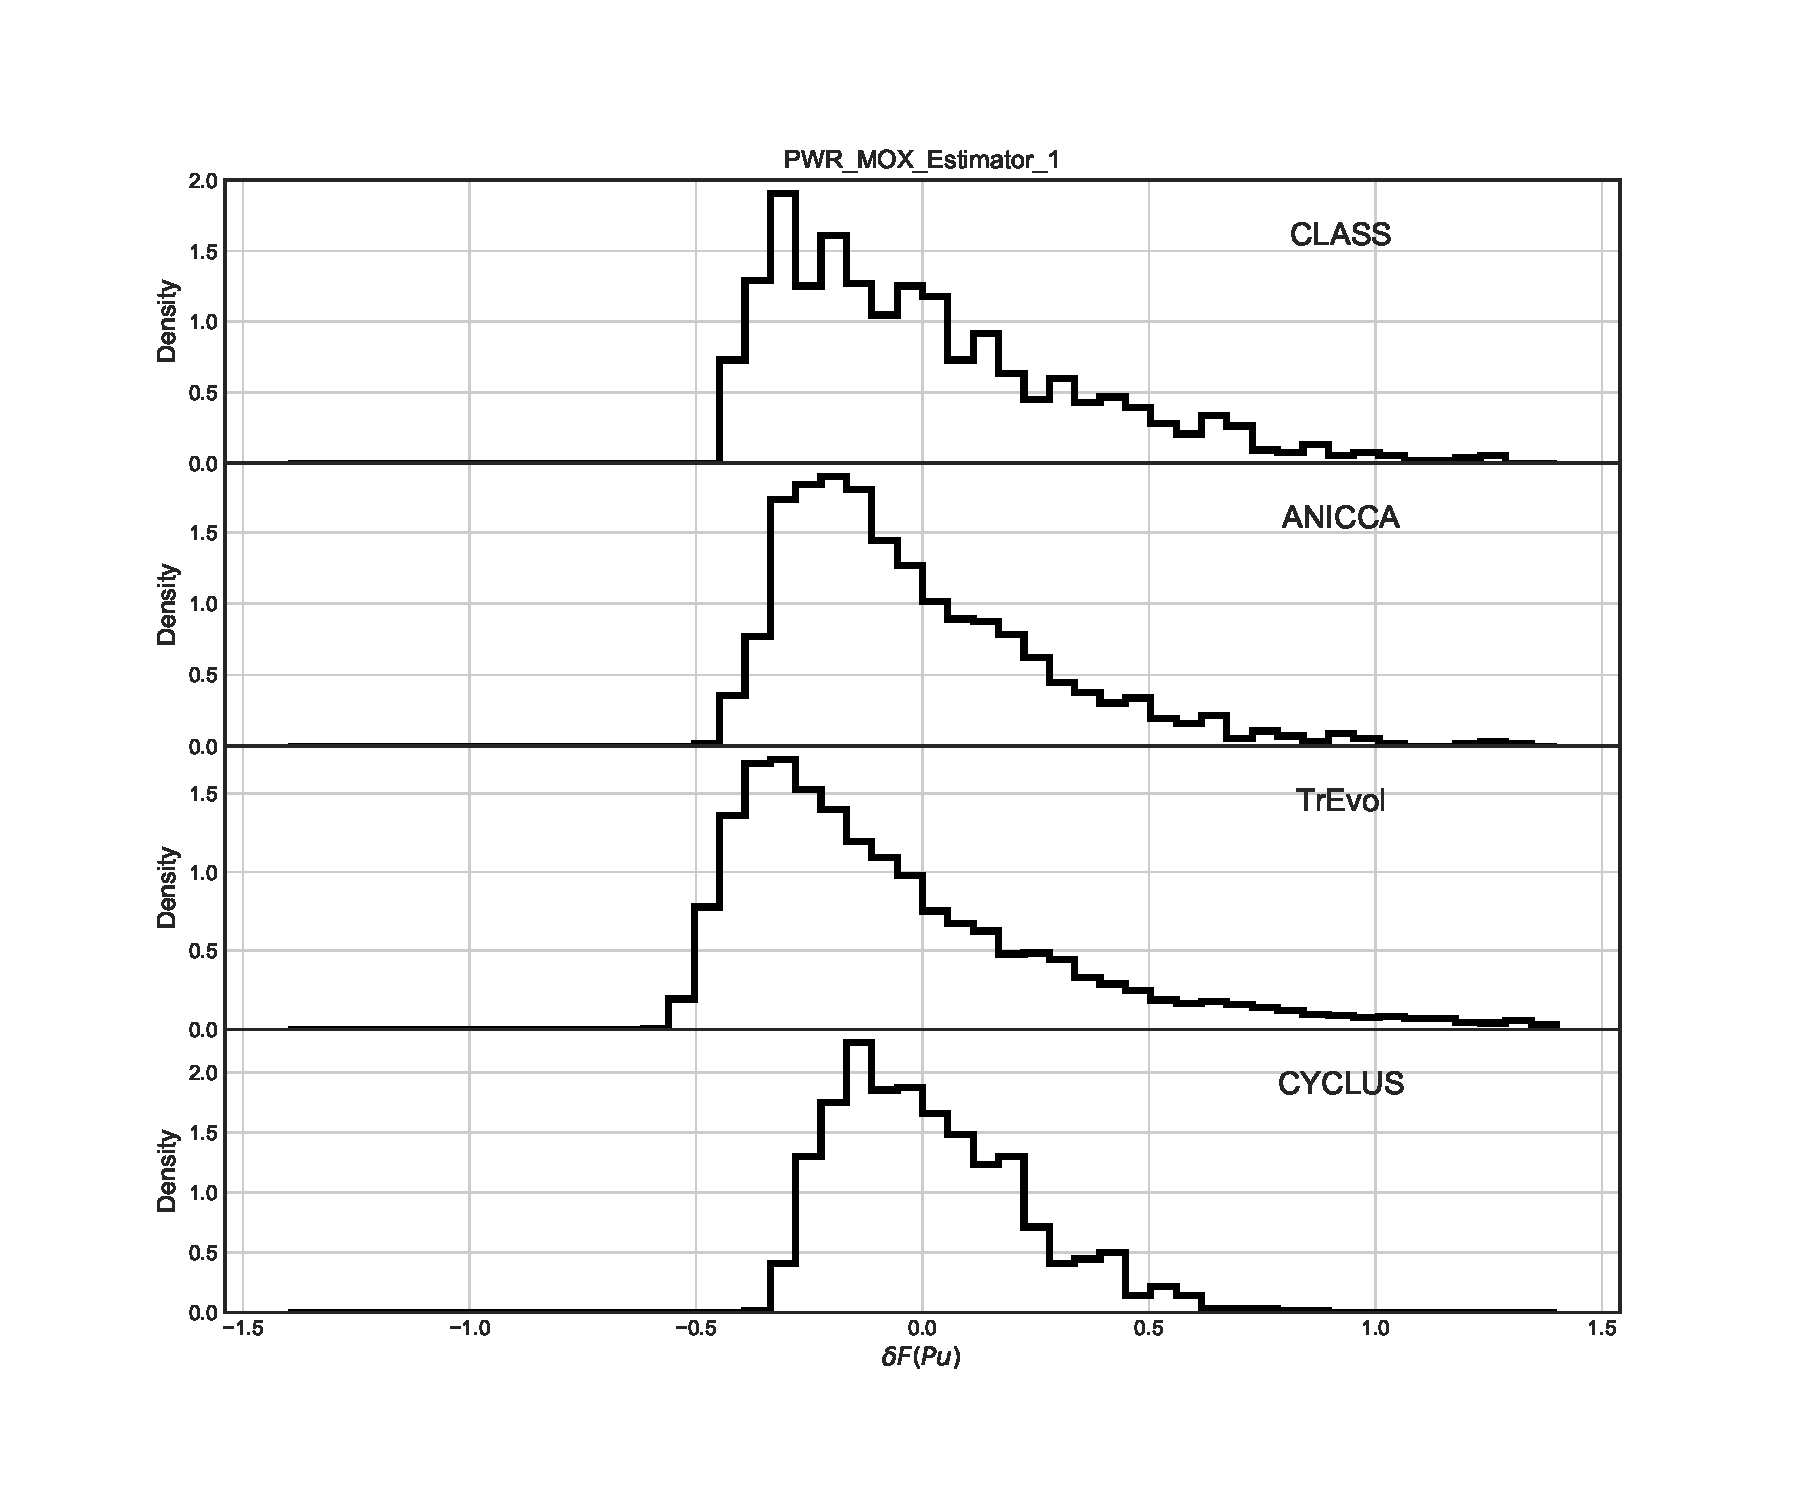
\includegraphics[width = 0.99\textwidth]{../../Feature_1/RAW_DATA/FIG/PWR_MOX_Estimator_1.pdf}
		\caption{Estimator 1 for PWR calculated with ANICCA, CLASS, CYCLUS and TrEVOL}
		\label{fig:Est1_PWR}
	\end{center}
\end{figure}

The standard deviation of the distribution is also a relevant quantity as it quantifies the dispersion of the calculation bias. A small standard deviation implies a narrow distribution and means small calculation biases due to the use of FF model. As we can see on the plot, none of the used software for this work shows a small standard deviation. This means that, in the range of the plutonium composition sampled, the use of a FF model induce strong calculation bias in the fresh MOX fuel plutonium fraction, hence strong bias in the mass of spent fuel that have to be reprocessed for the MOX fuel fabrication.

\paragraph{Ratio between plutonium consumption and plutonium at BOC}
Estimator 2 aims to quantify the amount of plutonium consumption regarding the plutonium mass at BOC. It measures the proportion of plutonium which is burnt during irradiation. Estimator 2 biases give an estimation of the total inventory precision calculation, no matter the location of the plutonium. 
Figure~\ref{fig:Est2_PWR} represents the different histograms of this estimator for the 4 codes used in this work. There are two trends in this plot: CYCLUS and CLASS shows limited biais (with a standard deviation of approximately XX as it can be seen in table~\ref{table:Est2_PWR}), whereas TR_EVOL and ANICCA calculates very strong biases. From this different behaviours, it is impossible to conclude on the FLM relevance for total inventory estimation. A limited biais (as seen with CYCLUS and CLASS) means that the use of a FF for plutonium enrichment at BOC may be sufficient for global inventory estimation. On the opposite, results from ANICCA and TR_EVOL tends to show that a FLM is necessary. 

\begin{figure}[h]
	\begin{center}
		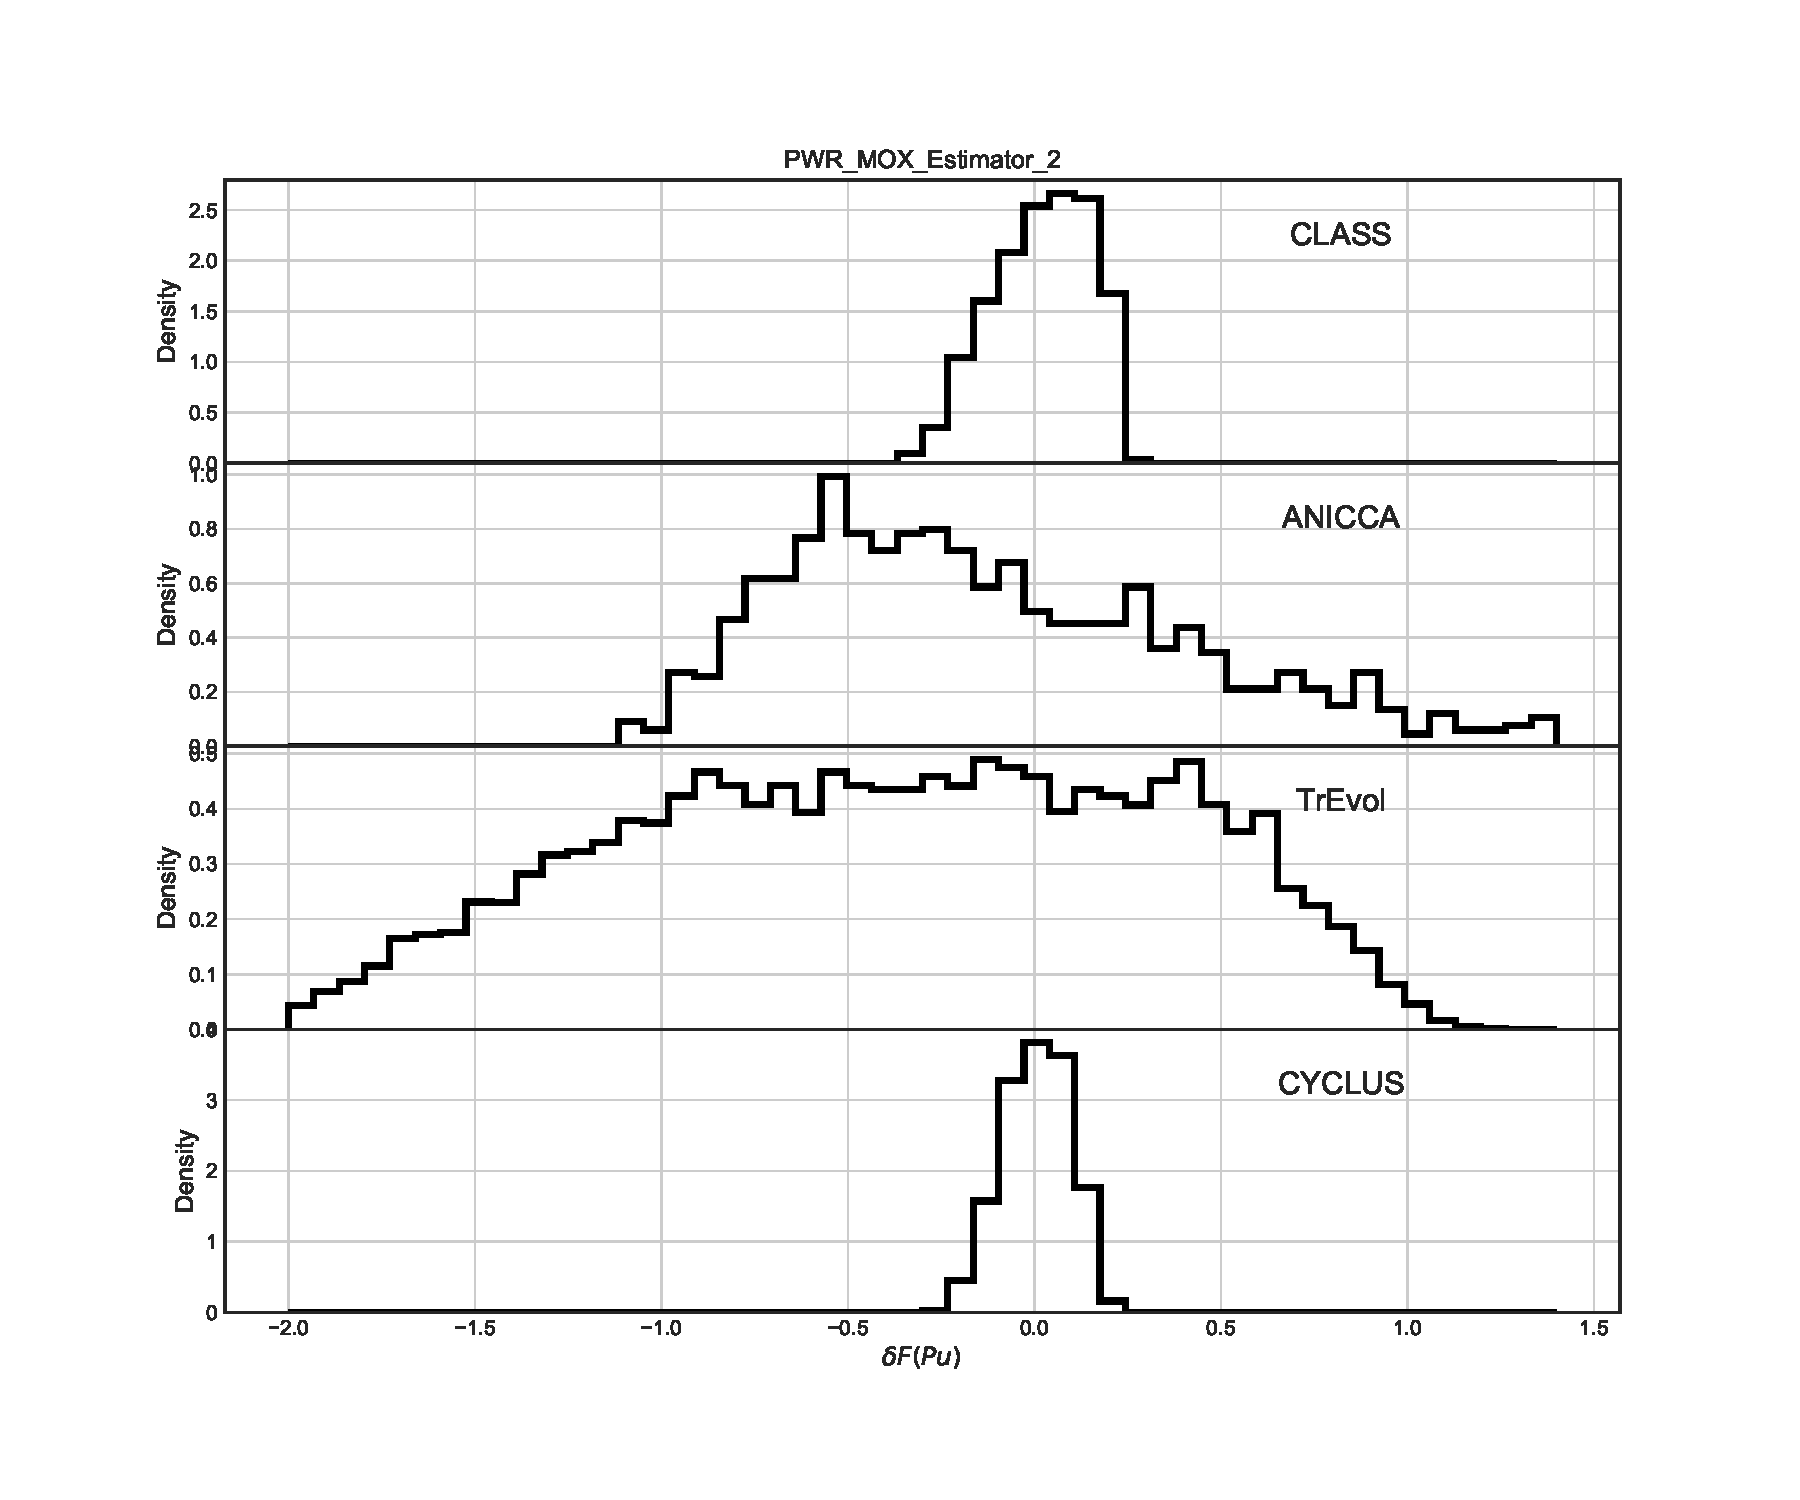
\includegraphics[width = 0.99\textwidth]{../../Feature_1/RAW_DATA/FIG/PWR_MOX_Estimator_2.pdf}
		\caption{Estimator 2 for PWR calculated with CLASS, CYCLUS and TrEVOL}
		\label{fig:Est2_PWR}
	\end{center}
\end{figure}

begin{table}[h]
	\begin{center}
		\begin{tabular}{|c||c||c|}
			\hline 
				CLASS & ANICCA & TR_EVOL & CYCLUS \\
			\hline
				XX & YY & ZZ && TT\\
		\end{tabular}
	\end{center}
	\label{table:Est2_PWR}
\end{table}

It has to be pointed out the fact that this estimator calculation (as for estimator 3 shown in the next paragraph) needs a depletion calculation. Figure~\ref{fig:PWR_MOX_FLM_Pu} shows that this depletion calculation is questionnable for some plutonium isotopic compositions with ANICCA and TR_EVOL. Those two software are used behond their validity domain and this is reflected in the very wide distribution of Estimator 2. The depletion calculation, innacurate for composition outside of the validity domain, adds some biases to the one brought by the FF model uses. The conclusions made with ANICCA and TR_EVOL has then to be consider with caution

\paragraph{Plutonium consumption rate}
Estimator 3 measures biases on the plutonium consumption rate calculation. As so, it measures the biases induced by a FF for plutonium enrichment at BOC on a global scale. It aims to quantify the global inventory evolution rate. 
Figure~\ref{fig:Est3_PWR} represents estimator 3 for CLASS, ANICCA, TR_EVOL and CYCLUS. Similar conclusion can be drawn as preivous section. CLASS and CYCLUS are in agreement as shows that the impact of using a FF may be limited, introducting 10\% bias on the total plutonium consumption rate. On the contrary ANICCA and TR_EVOL are also in agreement showing a much larger bias. The same caution of previous section should be pointed out: depletion calculation of the latest software are out of validity domain adding some uncertainty to the bias calculated by the use of FLM.       

\begin{figure}[h]
	\begin{center}
		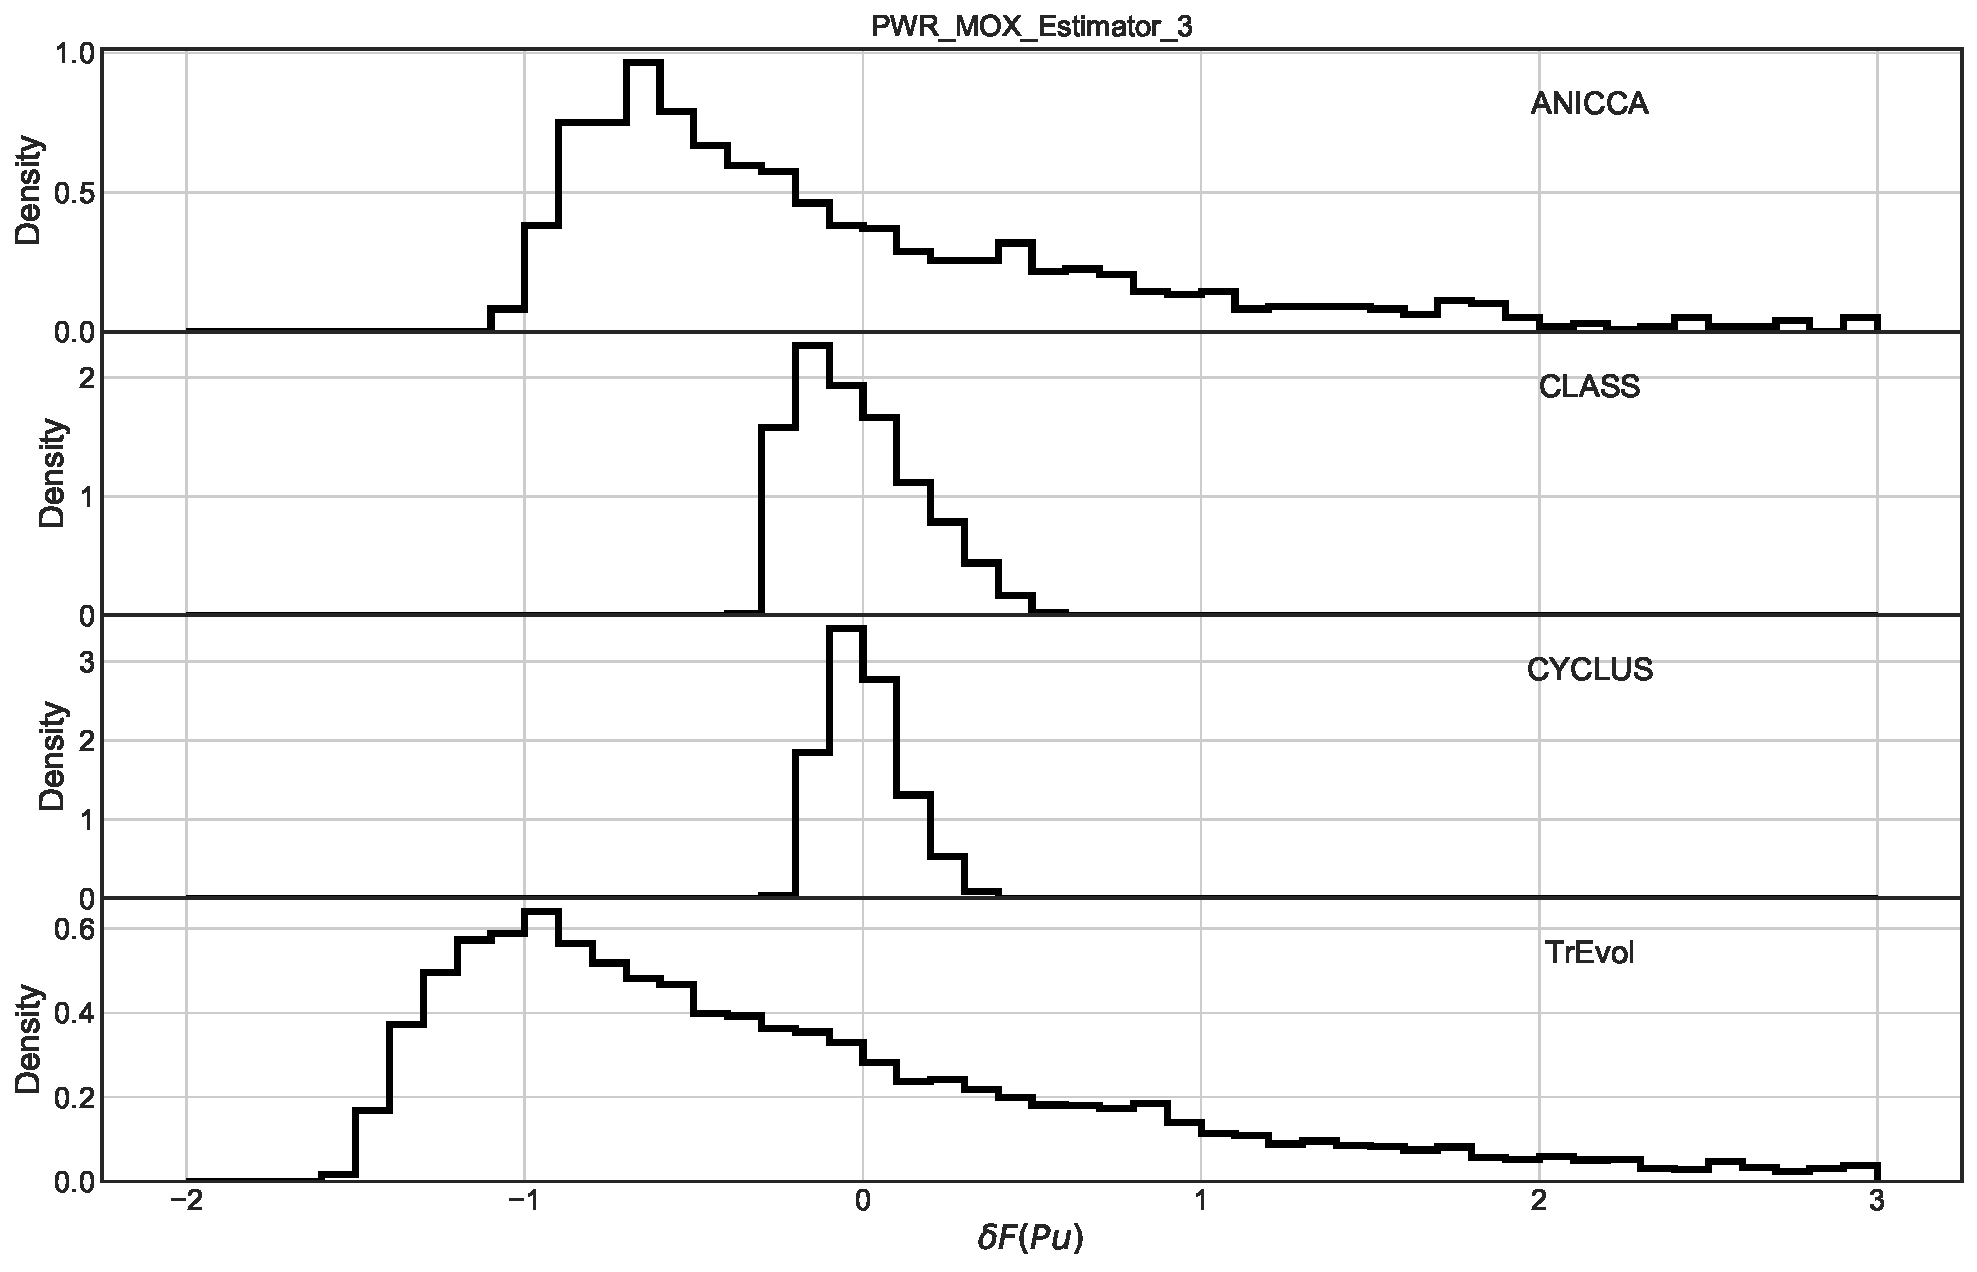
\includegraphics[width = 0.99\textwidth]{../../Feature_1/RAW_DATA/FIG/PWR_MOX_Estimator_3.pdf}
		\caption{Estimator 3 for PWR calculated with CLASS, CYCLUS and TrEVOL}
		\label{fig:Est3_PWR}
	\end{center}
\end{figure}

\subsection{Fast Sodium cooled Reactor}
\subsubsection{Output analyses}
Figure~\ref{SFR_MOX_FLM_Pu} represents the plutonium enrichment distribution at BOC (in black) and at EOC (in red) simulated with CLASS, JOSETTE and TR_EVOL. The different reactor models used for the different software explain the different behavior. CLASS simulates a breeder whereas TR_EVOL a simulate a burner and JOSETTE a break-even reactor. Plutonium mass evolution is then different for all those software. The purpose of this paper is not to compare software but to compare the use or not for each of those software. The fact that the reactor models shows different behavior reinforces conclusions drawn for the importance of FLM in fuel cycle simulators.     
\begin{figure}[h]
	\begin{center}
		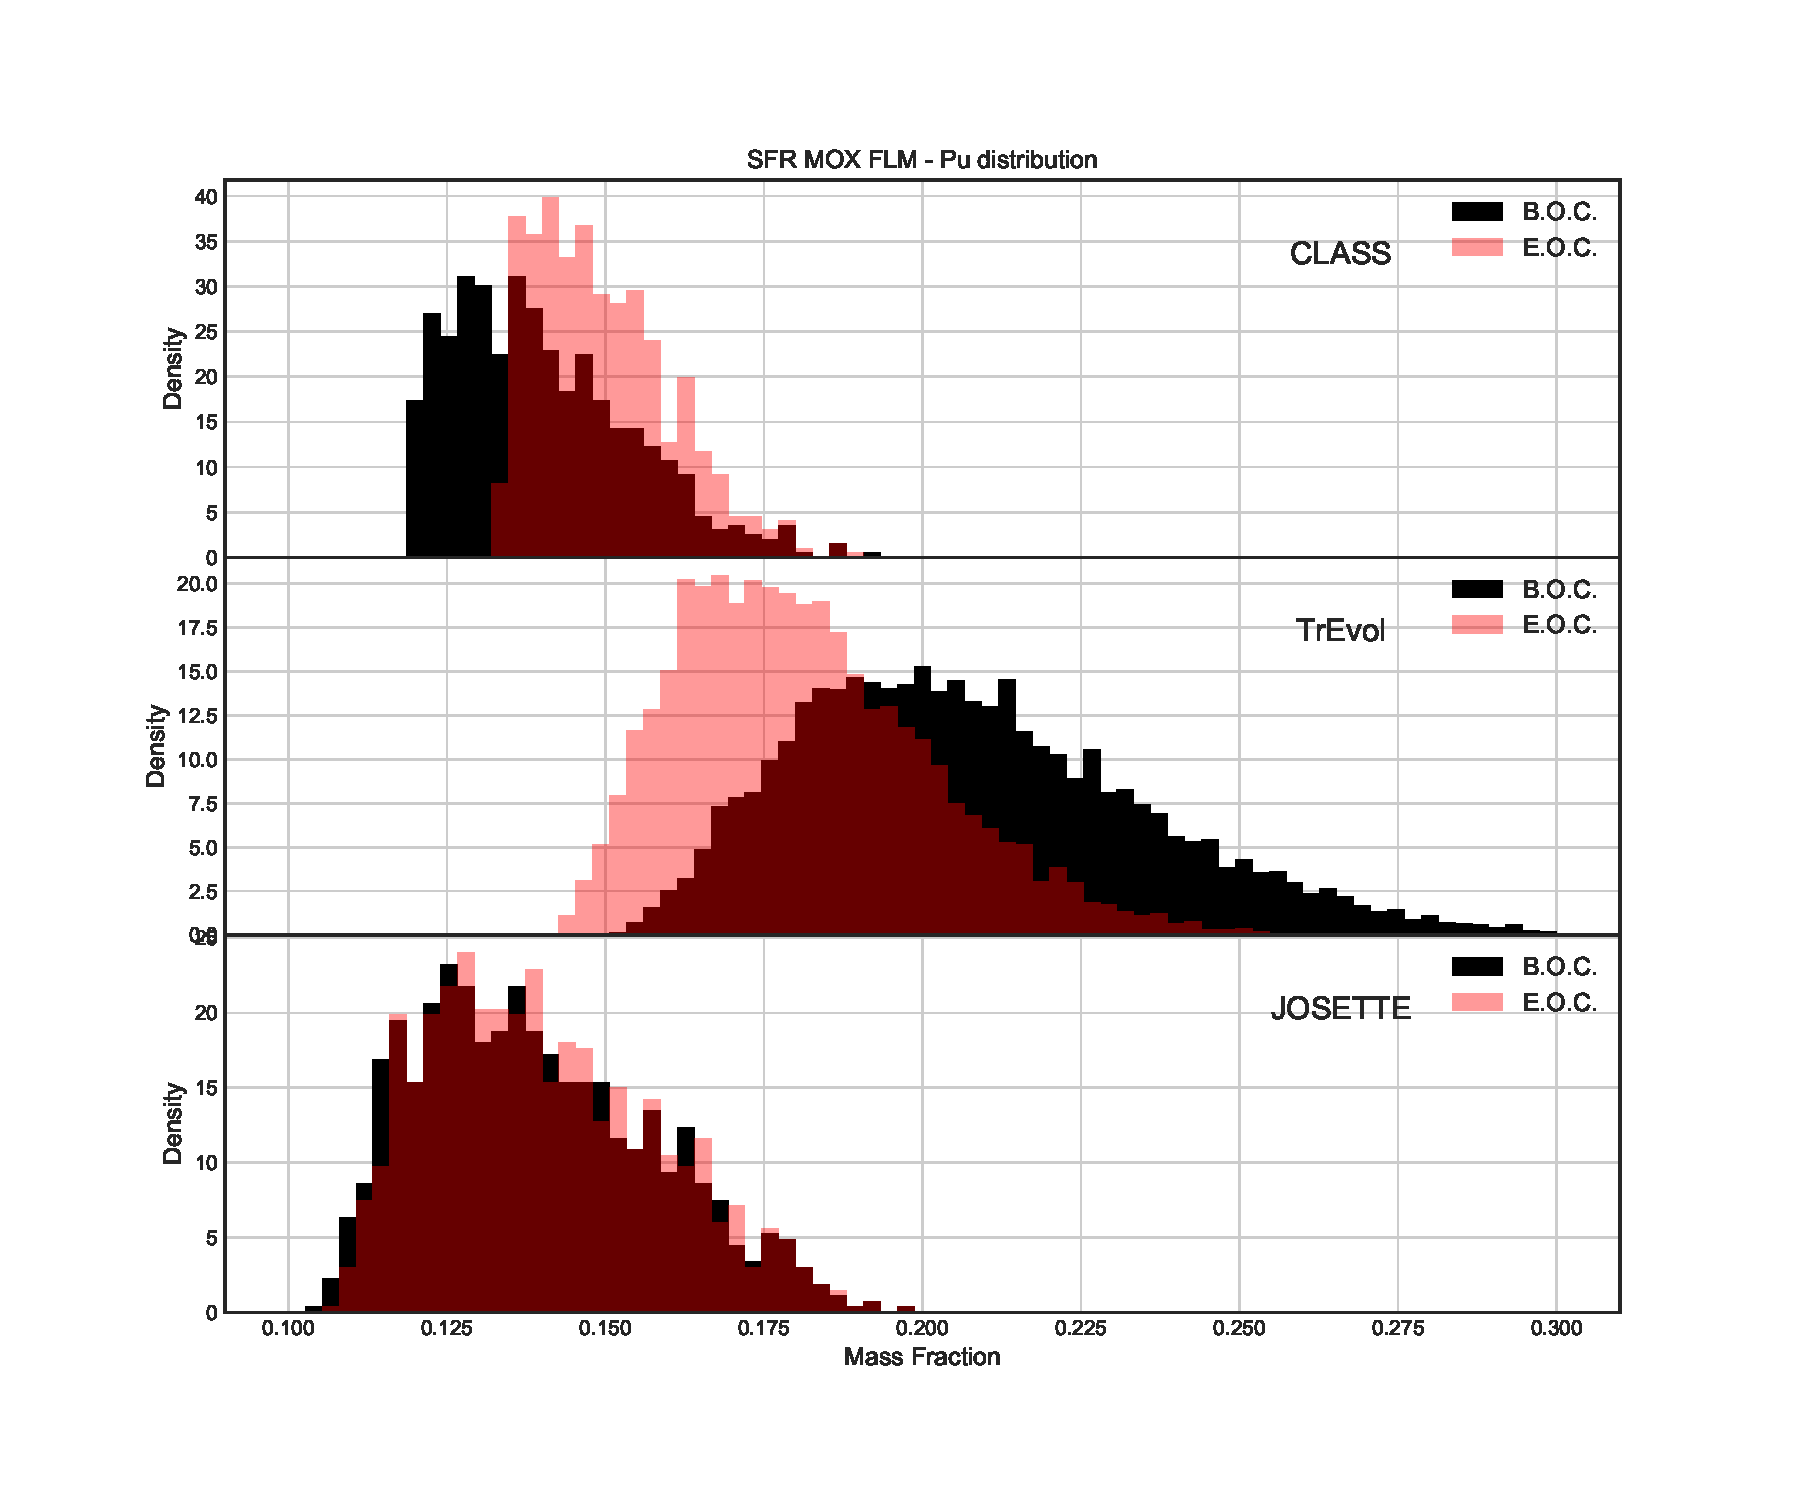
\includegraphics[width = 0.99\textwidth]{../../Feature_1/RAW_DATA/FIG/SFR_MOX_FLM_Pu.pdf}
		\caption{Code outputs for PWR scenario's calculations}
		\label{fig:SFR_MOX_FLM_Pu}
	\end{center}
\end{figure}

\subsubsection{Estimator's calculation}
\paragraph{Plutonium fraction at BOC}
Figure~\ref{fig:Est1_SFR} represents the estimator 1 calculated for Sodium Cooled Fast Reactors calculated with JOSETTE, TrEVOL and CLASS. Like for PWR, it shows the relative difference of plutonium enrichment with the use of a FLM in regards to a FF. Standard deviations of the difference distribution is given in Table~\ref{table:Est1Dev_SFR} for the different codes. All codes are in agreement even if CLASS slightly underestimate the FF impact on the plutonium needed for a SFR. The typical bias produced by the use of a FF is smaller than 25\% and is much lower than for PWR.   

\begin{figure}[h]
	\begin{center}
		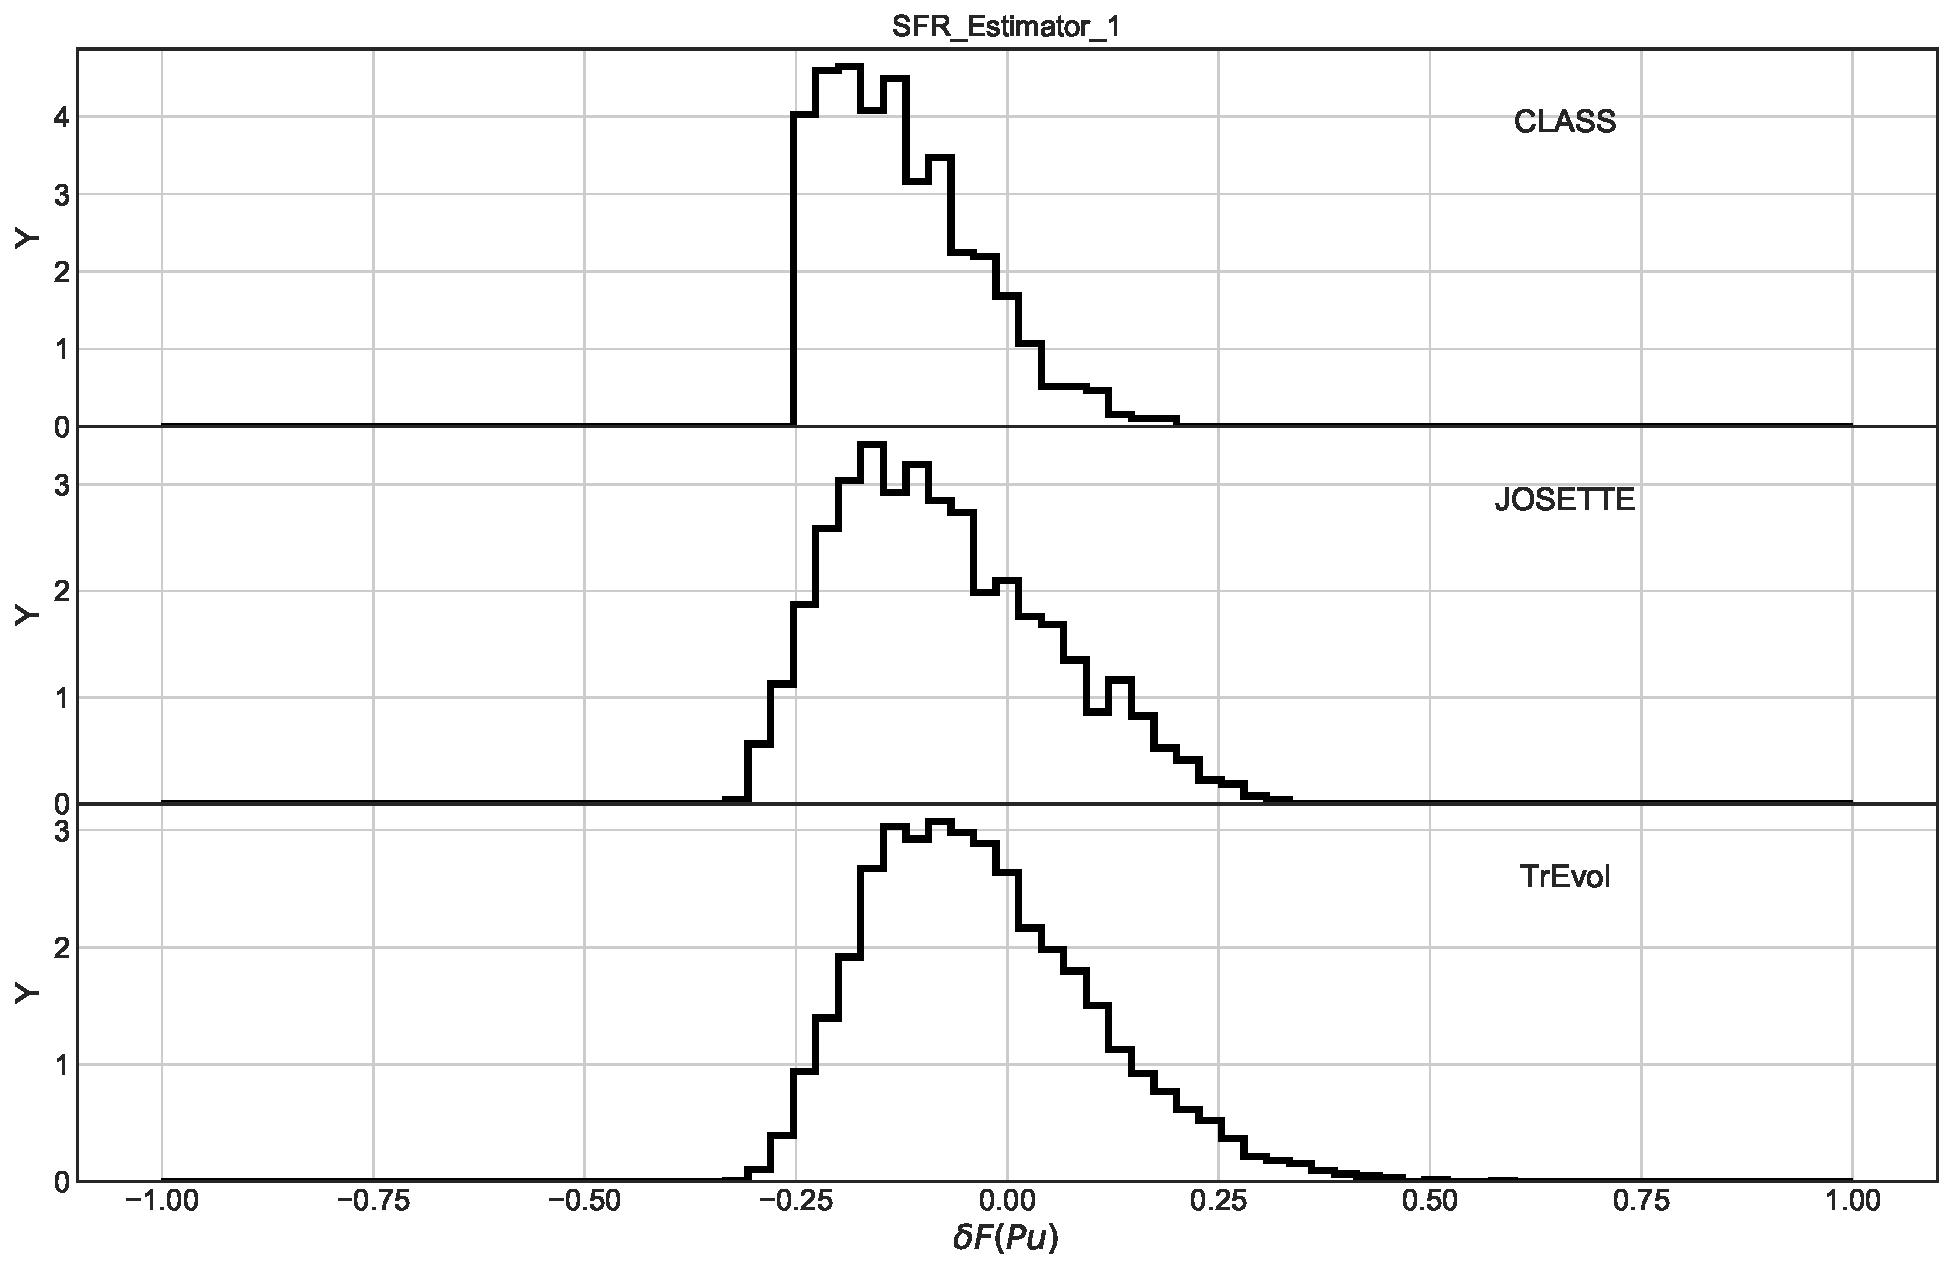
\includegraphics[width = 0.99\textwidth]{../../Feature_1/RAW_DATA/FIG/SFR_Estimator_1.pdf}
		\caption{Estimator 1 for SFR calculated with JOSETTE, TrEVOL, and CLASS}
		\label{fig:Est1_SFR}
	\end{center}
\end{figure}

\begin{table}[h]
	\begin{center}
		\begin{tabular}{|c||c||c|}
			\hline 
				JOSETTE & TrEVOL & CLASS \\
			\hline
				XX & YY & ZZ \\
		\end{tabular}
	\end{center}
	\label{table:Est1Dev_SFR}
\end{table}

The estimation of spent fuel mass that have to be reprocessed for SFR fresh fuel composition using a FF for plutonium enrichment is then estimated with a bias smaller than 10\% no matter the SFR behavior (breeder, burner or break-even).  

\paragraph{Ratio between plutonium consumption and plutonium at BOC}
Estimator 2.b aims to calculate the plutonium production or consumption on the global level of the fleet. It estimates the absolute difference on breeding ratio when simulation are made with a FF or with a FLM. CLASS and TR_EVOL shows similar results and calculate biases induced by the FF method up to 0.1. JOSETTE calculations shows a narrower distribution, probably due to the fact that SFR simulated with JOSETTE are all break-even.   

\begin{figure}[h]
	\begin{center}
		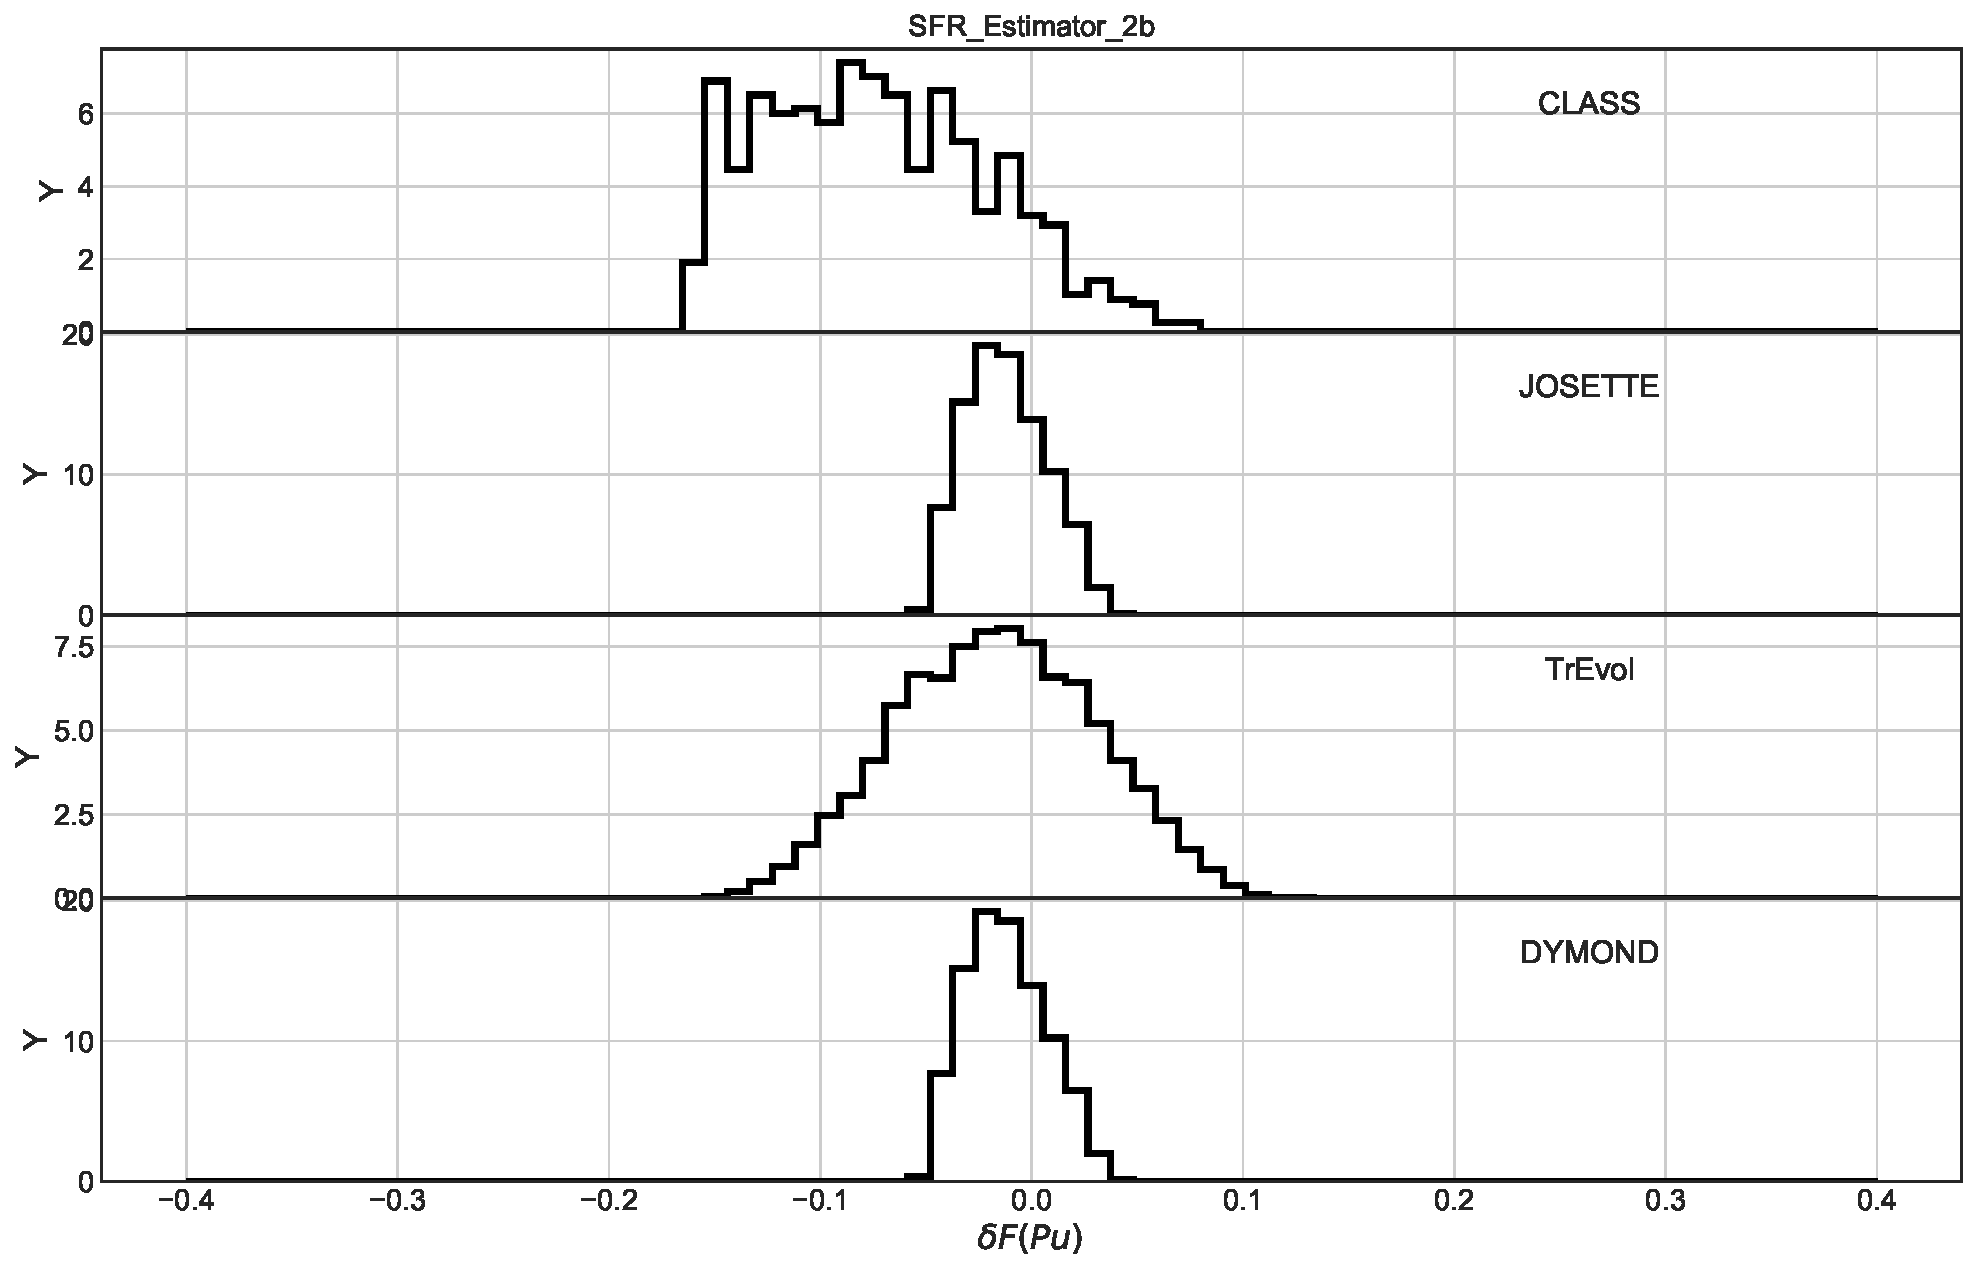
\includegraphics[width = 0.99\textwidth]{../../Feature_1/RAW_DATA/FIG/SFR_Estimator_2b.pdf}
		\caption{Estimator 2.b for SFR calculated with JOSETTE, TrEVOL, and CLASS}
		\label{fig:Est2_SFR}
	\end{center}
\end{figure}
